\documentclass[a4paper,twoside,11pt, fleqn]{article}
\usepackage{a4wide,graphicx,fancyhdr,amsmath,amssymb}
\usepackage{listings}
\usepackage{color}
\usepackage{dirtree}
\usepackage{subcaption}

%matlab 
\usepackage[]{mcode}

%----------------------- Macros and Definitions --------------------------

\setlength\headheight{20pt}
\addtolength\topmargin{-10pt}
\addtolength\footskip{20pt}

\newcommand{\N}{\mathbb{N}}
\newcommand{\ch}{\mathcal{CH}}

\newcommand{\solution}[1]{\noindent{\bf Solution to Exercise #1:}}

\fancypagestyle{plain}{%
\fancyhf{}
\fancyhead[LO,RE]{\sffamily\bfseries\large technische universiteit eindhoven}
\fancyhead[RO,LE]{\sffamily\bfseries\large 2IN35 VLSI}
\fancyfoot[LO,RE]{\sffamily\bfseries\large department of mathematics and computer science}
\fancyfoot[RO,LE]{\sffamily\bfseries\thepage}
\renewcommand{\headrulewidth}{0pt}
\renewcommand{\footrulewidth}{0pt}
}

\pagestyle{fancy}
\fancyhf{}
\fancyhead[RO,LE]{\sffamily\bfseries\large technische universiteit eindhoven}
\fancyhead[LO,RE]{\sffamily\bfseries\large 2IN35 VLSI}
\fancyfoot[LO,RE]{\sffamily\bfseries\large department of mathematics and computer science}
\fancyfoot[RO,LE]{\sffamily\bfseries\thepage}
\renewcommand{\headrulewidth}{1pt}
\renewcommand{\footrulewidth}{0pt}

\def\addsquare#1{\tikz\node[draw]{#1};} 

%-------------------------------- Title ----------------------------------

\title{\vspace{-\baselineskip}\sffamily\bfseries Assignment 4}
\author{
	Rick Veens \qquad Studentno: 0912292\\
	\texttt{r.veens@student.tue.nl}
	\and
	Barry de Bruin \qquad Studentno: 0919605\\
	\texttt{e.d.bruin@student.tue.nl}
	\and
	\texttt{Group 7}
}

\date{\today}

\setlength\parindent{0pt}

%--------------------------------- Text ----------------------------------

\begin{document}
\maketitle
\newpage

\tableofcontents

\newpage

\section{Requirements}
\subsection{Analysis of requirements}
\section{System architecture}
\section{Design choices}
\section{Functional correctness}
\section{Resource usage}
\section{System throughput and latency}
\section{Offline project results}
\subsection{256 Streams}
\subsection{1024 Streams}

\section{Appendix A: Matlab coefficients script}
\begin{lstlisting}
% Put this in a file named coef_generate_matlab.m, then call it 
% while you are in the file directory. It will write the coefficients
% to the coef.txt file and also return them.

function [y] = coef_generate_matlab(L)
        % make sure that coefficients sum to 1
        y = coef_gen(L);
        y = y/sum(y);

        % quantize and round to nearest integer
        y = y * 160;
        y = round(y*(2^15)); 
             
        % convert to signed int filter coeff
        y = int16(y);
        y = hex(fi(y, 1, 16, 0)); %1 stands for signed, 16 bit out
        
        dlmwrite('coef.txt',y,''); %create file, with no delimiter ''      
end

function [y] = coef_gen(L)
    % generate 4*L coefficients and start at 0 instead of 1 *stupid matlab*
    for n = 1:4*L
            y(n) = lanczos2(((n-1)/L) -2);
    end
end

function y = lanczos2(t)
    if(t <= -2 || t >= 2)
        y = 0;
    else
        y = sinc(t).*sinc(t/2);
    end
end
\end{lstlisting}

Figure~\ref{fig:frq} shows the frequency response of the FIR filter that is generated with help of the matlab code from appendix A.

\begin{figure}[h]
	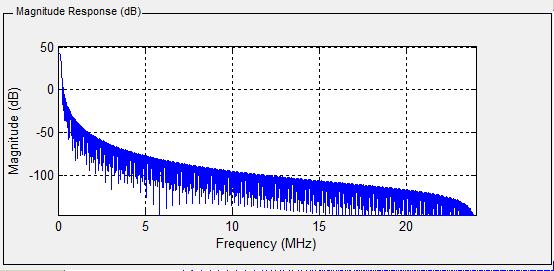
\includegraphics[scale=0.67]{Images/frequencyplot}
    \caption{Interpolation filter frequency domain (Matlab)}
    \label{fig:frq}
\end{figure}

\newpage
\section{Appendix B: Verilog Code}
File: filter.v.
\begin{lstlisting}[language=Verilog]

\end{lstlisting}

\end{document}
